\documentclass[12pt,a4paper]{article}
%% ntts2021abstract_template.tex
%% TEMPLATE FOR NTTS 2021 CONFERENCE

\def\thisfile{biblio}

%% WHAT IS YOUR PAPER ABOUT: PUT YOUR TITLE HERE
\def\thetitle{
\textbf{Democratization of time-varying coefficients models}
}

%% TELL US MORE... THROUGH KEYWORDS!
\def\thekeywords{
\textit{Long Time Series, structural breaks, Reg-Arima models, Calendar correction, Forecasting.}
}
% il semble qu'il faut mettre des mots qui ne figurent pas dans le titre...

%% PLEASE KEEP AT LIST THESE SETTINGS
\def\thepaperheight{29.9cm} 	% original: {11.99in}
\def\thepaperwidth{21.08cm} 	% 		{8.3in}
\def\theleft{2.79cm} 			% 		{1.1in}
\def\theright{2.99cm} 			%		{1.18in}
\def\thetop{1.7cm} 			% 		{0.51in}
\def\thebottom{1.6cm} 		% 		{0.71in}
\def\theheadheight{2.54cm} 	% 		(1in}

\usepackage[
   a4paper,
   paperheight=\thepaperheight,
   paperwidth=\thepaperwidth,
   left=\theleft,
   right=\theright,
   top=\thetop,
   bottom=\thebottom,
   headheight=\theheadheight
]{geometry} % in particular, do not change the dimensions of the document

\usepackage{fancyhdr}

%\cfoot{ {\fontsize{8pt}{9.6pt}\selectfont 6\par}}

%% NO HEADING...
%%\fancyhead[RE]{\headreport}
%%\fancyhead[RO,LE]{\bfseries\thepage}
%%\fancyhead[LO]{\nouppercase{\rightmark}} %{\markright} %{\sectionmark}

\pagestyle{fancy}
\fancyhf{}

% you can use hyperref as set below once the colorboxes are gone...
% \usepackage[pdfauthor={\theauthors}, pdftitle={\thetitle}]{hyperref}
% otherwise simply stick to that one
\usepackage{hyperref}

\hypersetup{colorlinks=true,       % false: boxed links; true: colored links
    % linkcolor=blue,          % color of internal links
    citecolor=red,        % color of links to bibliography
    filecolor=magenta,      % color of file links
    urlcolor=cyan           % color of external links
}
%% or:
% \usepackage[hidelinks]{hyperref} % make links black

\usepackage{sectsty}
\usepackage{setspace}

\renewcommand{\headrulewidth}{0pt}
\setlength{\topsep}{0pt}\setlength{\parindent}{0pt}

\renewcommand{\arraystretch}{1.3}

%% depths for Sections 
% 1) Section
% 1.1) SubSection
% 1.1.1) SubSubSection
% 1.1.1.1) Paragraph
\setcounter{tocdepth}{4}
\setcounter{secnumdepth}{4}

% depths for nested lists created by \begin{enumerate}
\usepackage{enumitem}
\setlistdepth{9}
\renewlist{enumerate}{enumerate}{9}
	\setlist[enumerate,1]{label=\arabic*)}
	\setlist[enumerate,2]{label=\alph*)}
	\setlist[enumerate,3]{label=(\roman*)}
	\setlist[enumerate,4]{label=(\arabic*)}
	\setlist[enumerate,5]{label=(\Alph*)}
	\setlist[enumerate,6]{label=(\Roman*)}
	\setlist[enumerate,7]{label=\arabic*}
	\setlist[enumerate,8]{label=\alph*}
	\setlist[enumerate,9]{label=\roman*}
\renewlist{itemize}{itemize}{9}
	\setlist[itemize]{label=$\cdot$}
	\setlist[itemize,1]{label=\textbullet}
	\setlist[itemize,2]{label=$\circ$}
	\setlist[itemize,3]{label=$\ast$}
	\setlist[itemize,4]{label=$\dagger$}
	\setlist[itemize,5]{label=$\triangleright$}
	\setlist[itemize,6]{label=$\bigstar$}
	\setlist[itemize,7]{label=$\blacklozenge$}
	\setlist[itemize,8]{label=$\prime$}

% that's for generating directly PDF documents using pdfLaTex instead of LaTex alone
\newif\ifpdf\ifx\pdfoutput\undefined\pdffalse\else\pdfoutput=1\pdftrue\fi
\newcommand{\pdfgraphics}{\ifpdf\DeclareGraphicsExtensions{.pdf,.png,.tif,.jpg}\else\fi}

%% KEEP THIS FOR THE EXAMPLES BELOW TO RUN...OR RUN YOUR OWN
% \usepackage[boxed]{algorithm2e}
\usepackage{algorithm}
%\usepackage{algorithmic}
\usepackage[noend]{algpseudocode}
\makeatletter\def\BState{\State\hskip-\ALG@thistlm}\makeatother
% force indenting 
\newcommand{\forceindent}{\leavevmode{\parindent=1em\indent}}

%% DEAL WITH THE BIBLIOGRAPHY

% that's what we use here for the bibliography
\usepackage[numbers]{natbib}
% see https://gking.harvard.edu/files/natnotes2.pdf
\newcommand*{\doi}[1]{DOI: \href{https://doi.org/\detokenize{#1}}{\detokenize{#1}}} 
\newcommand*{\arxiv}[1]{arXiv: \href{https://arxiv.org/abs/\detokenize{#1}}{\detokenize{#1}}} 

%% If you are compiling using biblatex
%\usepackage[
%    backend=biber,
%    style=authoryear,
%    natbib=true,
%    url=true, 
%    doi=true,
%    eprint=false, 
%    sorting=ynt
%]{biblatex}
%\addbibresource{\thisfile.bib}

%% THANKS!

%% SUGGESTED PACKAGES - YOUR CALL 

\usepackage[utf8]{inputenc}
\usepackage[T1]{fontenc}

\usepackage{amsmath}
\usepackage{latexsym}
\usepackage{amsfonts}
\usepackage[normalem]{ulem}
\usepackage{array}
\usepackage{amssymb}

\ifpdf
\usepackage[pdftex]{graphicx}
\else
\usepackage{graphicx}
\fi

%\graphicspath{
%
%}

\usepackage{float}
%\usepackage{subfloat}
\usepackage{subfig}
\usepackage{caption}
% \usepackage[list=true]{subcaption} % cannot be used conjointly with subfig
\usepackage{wrapfig}
\usepackage{wasysym}
\usepackage[svgnames,table,rgb]{xcolor}
\usepackage{longtable} % long tabulars
\usepackage{adjustbox}
\usepackage{alltt} % verbatim 
\usepackage{changepage}
\usepackage{hhline}
\usepackage{multicol}
\usepackage{tabto}
\usepackage{multirow}
\usepackage[utf8]{inputenc}
\usepackage[top=2 cm, bottom=2 cm, left=2.5 cm, right=2.5 cm]{geometry}
\usepackage{amsfonts,amsmath,amsthm,amssymb,stmaryrd} 
%\usepackage{amsmath}
%\usepackage{ragged2e}
%\usepackage{makecell}
%\usepackage[toc,page]{appendix}

% usually not necessary if you include figures as png/jpg...
\usepackage{pgfplots}
\usepackage{tikz}
\usetikzlibrary{arrows,backgrounds,snakes}
\usepackage{fontawesome5}
\usepackage{animate, dsfont, here, xspace}

\urlstyle{same}


 %% HEADER
\title{
\vspace{-5ex}
\thetitle
\vspace{-2ex}
}
\author{
\theauthors
\vspace{-5ex}
}
\date{}


%% YOUR DOCUMENT STARTS HERE

\begin{document}
\cfoot{\thepage} % keep pages numbered

%% PLEASE KEEP THIS FORMATTING
\sectionfont{\large\textsc}
%\sectionfont{\large\MakeUppercase}
%%

\maketitle
{\fontsize{10pt}{12.0pt}\selectfont \textbf{\uline{Keywords}:} \thekeywords\par}\par


\section{Introduction}

In official statistics, linear regressions are everywhere: trading-day adjustments and forecasting models rely on RegARIMA models and macroeconomic models use error correction models. These methods generally provide reliable results and a straightforward interpretation.\\

However, they assume that the relationships between the variables are fixed in time: this assumption may make sense in the short term, but is generally no longer valid when the models are estimated over a long period, which leads to sub-optimal modelling.

Many authors have studied time-varying coefficients (from piece-wise regression to state-space models estimated by neural networks, see for example \cite{rangapuram2018deep}), but practical applications of these methods are note easily reproducible for the average user and even more difficult to set up in production.

The goal of this study is to provide a new \faIcon{r-project} tool to easily select, implement and test time-varying regressions in the aforementioned cases. This tool will particularly appeal to data analysts in official statistics branch but could also prove useful to any statistician using \faIcon{r-project}. 

\section{Methods}

\subsection{Classical regression and testing for breaks}
In this section we outline a range of methods allowing to estimate time varying coefficients.
The model can generally be written as:
\[
y_t=\beta_t X_t+\varepsilon_t
\]
with \(y_t\) the observed dependent variable at time \(t\), \(X_t\) a set of covariates and \(\varepsilon_t\) the disturbance at time \(t\).

The classical linear regression assumes that \(\beta_t=\beta\) at all times \(t\) 
\subsubsection{Testing the stability of the coefficients}
Several tests can be used to test this hypothesis.
For example, \citet{hansen1992testing} proposes a test of constant parameters against the alternative that the parameters follow a martingale (simple structural breaks as well as random walk parameters).
\citet{bai2003computation} propose an efficient algorithm to test multiple structural breaks and detect the associated breakdates.
Both cannot be used in trading-day adjustment models where the error follows a SARIMA model, thus \citet{abs2006} proposed a different approach to test the constancy of the coefficients.

\subsubsection{Piece-wise regression}
The first and simpler model is the Piece-wise regression: the regressors are split according to the dates of the break.
For example for a full structural break\footnote{The model can be easily rewritten to take into account partial structural break in a subset of the covariates.} at a single date \(T_1\) (with no break in the variance), the model would be:
\[
y_t=\beta_1 X_t \mathds 1_{(t\leq T_1)} + \beta_2X_t\mathds 1_{(t>T_1)}+\varepsilon_t
\]
This is the model used in \citet{bai2003computation}.
It assumes that a sudden break happens on specific dates.
In that case the reason of the break can often be known (change in the methodology, etc.).
However, in most cases, it is more realistic to assume that the relationships between variable change slowly over time rather than suddenly, hence the need for time varying parameters.

\subsection{Time-varying parameter models}

\subsection{Rolling window estimations}

The simplest time-varying parameter model is based on ``rolling windows'': the estimation is done using a fixed number of observations (``bandwidth'').
The length of the window can be specified by the user or selected with some statistical procedures as cross-validation.
The date at which the estimates will be affected also has to be specified: it can be the last date or the middle date of the window but it requires a strategy to estimate the missing observations.
This method can also be extended using local polynomial kernel estimators: the coefficient is assumed to be locally polynomial\footnote{The simpler case is assuming that the coefficient is locally constant (Nadaraya-Watson estimator).} and the estimation is done using weighted local regression (see for example \citet{tvReg} for its implementation in \faIcon{r-project}).

One of the drawbacks of this approach is that all the coefficients are moving.
A two-step procedure might be done: the model is identified (detection of outliers and selection of the ARIMA model) and estimated using the full sample for the fixed regressors.

\subsection{State-space framework}

The last method studied in this paper uses the state-space modelling, assuming that the coefficients are random walks, as detailed in \citet{ch7HBSA} when dealing with time-varying trading-day corrections.

\section{Results}


The different methods are compared with a linear regression that can be used to nowcast the quarterly growth of the French industrial production of the other manufacturing sector (C5).
The explanatory variables are:

\begin{itemize}
\item
  The growth overhang in the first month of the quarter of the industrial production index.
\item
  From the INSEE monthly business tendency survey in industry: indicator of the business climate at the third month of each quarter, the level of overall order books at the second month of each quarter and the personal production expectations, in difference, at the third month of each quarter;
\item
  From the Banque de France monthly business tendency survey in industry: the production capacity utilization rate, in difference, at second month of each quarter.
\end{itemize}

\begin{figure}[H]
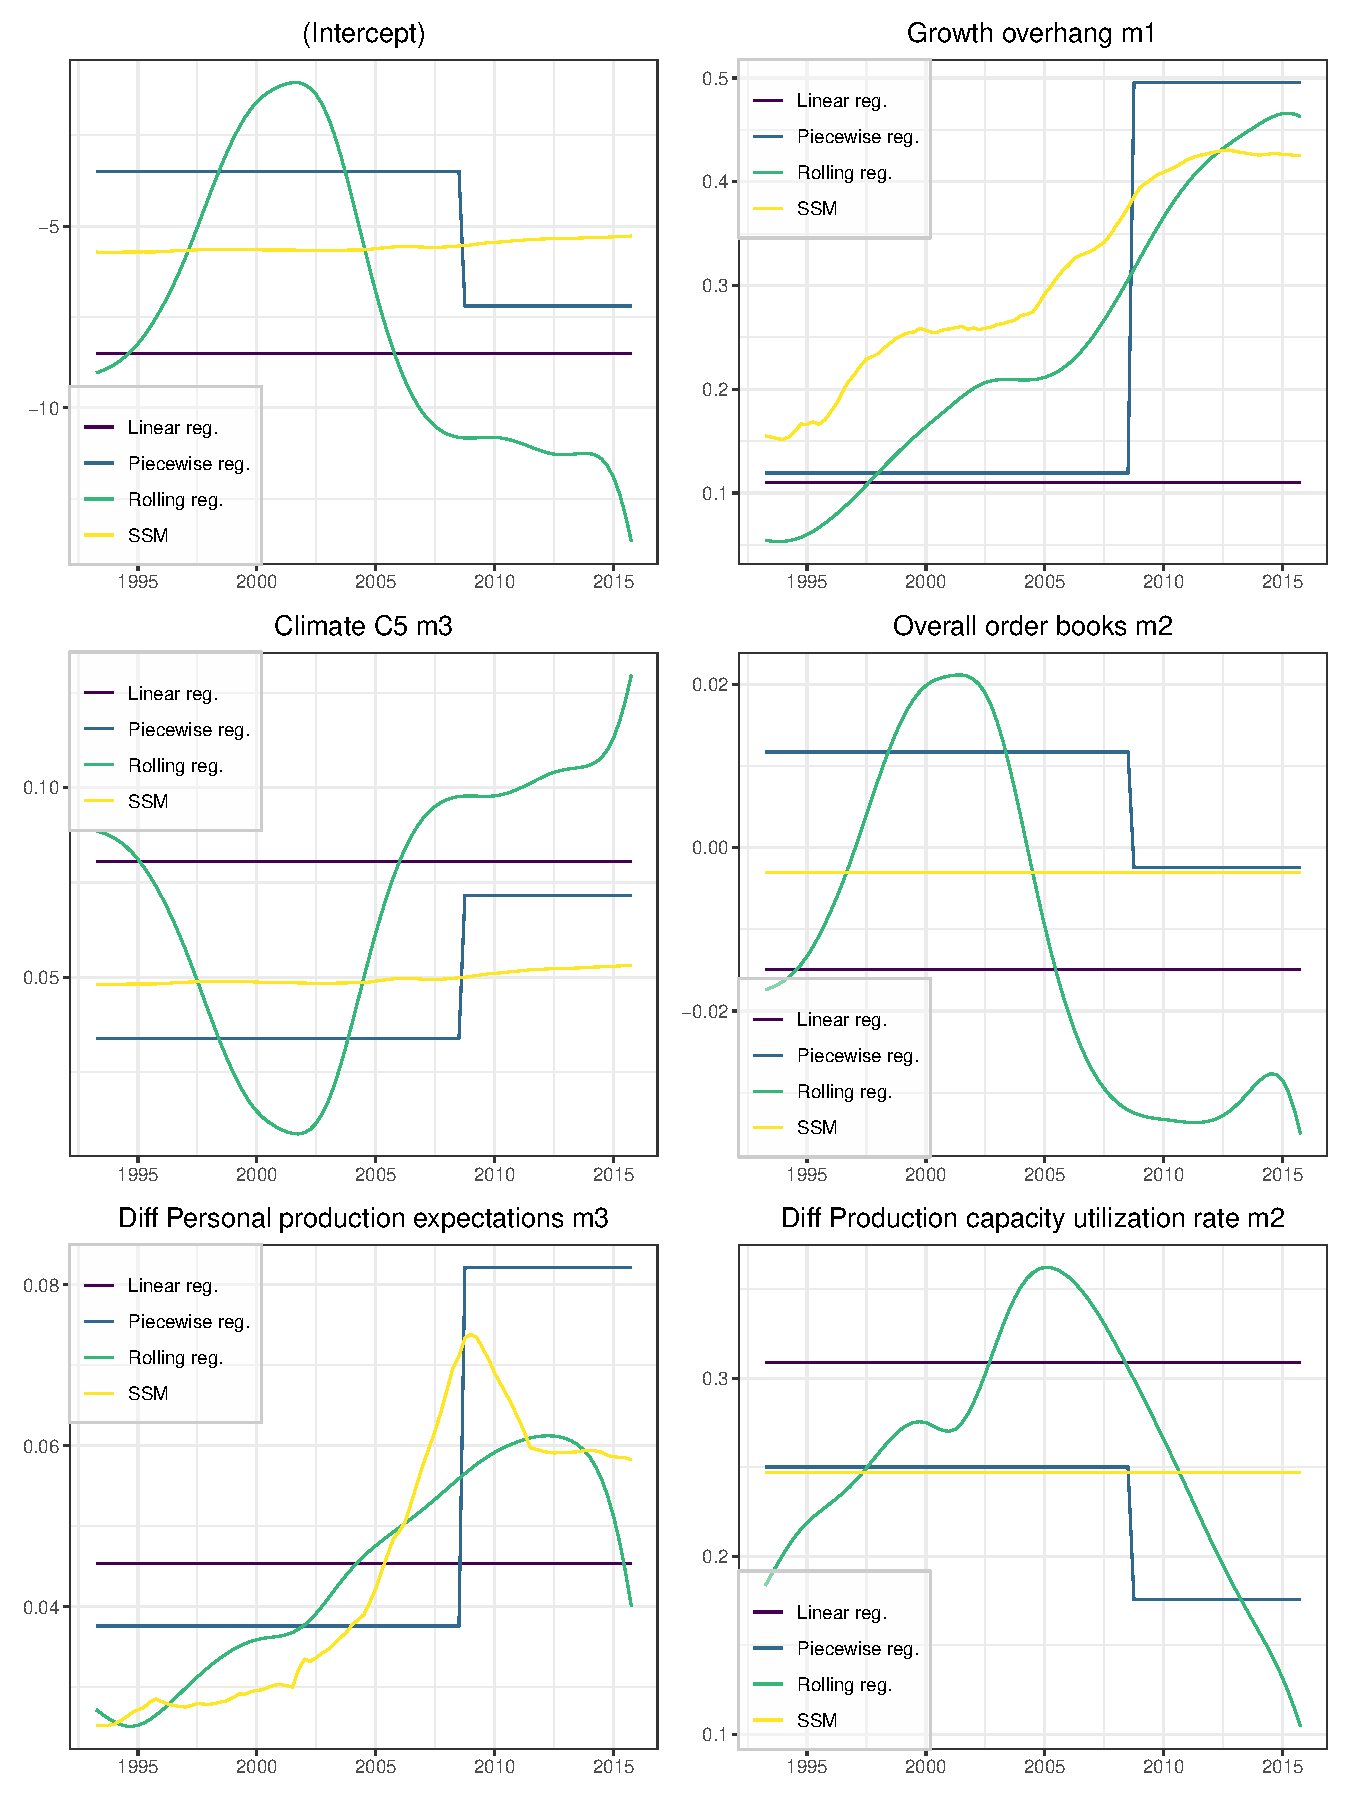
\includegraphics[width=1\linewidth]{img/example} \caption{Estimation of the coefficients of a linear model to forecast quarterly growth of the French industrial production of the other manufacturing sector (C5) with a simple regression, a piece-wise regression, a rolling regression and a state-space model.}\label{fig:example}
\end{figure}

The model is estimated from 1993Q1 to 2015Q4.
In the simple regression, the residuals are independent, homoskedastic and normal.
The \citet{bai2003computation} methodology detects one breakpoint in 2008Q3 and the \citet{hansen1992testing} test reject the hypothesis of constancy of parameters for the growth overhang and the personal production expectations.


Figure \ref{fig:example} shows the different estimates with the different method\footnote{
  For the rolling regression we assume that the coefficient is locally constant, an Epanechnikov kernel is used and the bandwidth is detected minimizing cross-validation.}.
Unsurprisingly, the results are different between across methods.
The estimates of the piece-wise regression might be subject to high revisions because few points are used to estimate the coefficients after the break.
Rolling regressions lead to high volatility in the estimates, probably due to the size of the bandwidth.
State-space models lead to time-varying coefficients only for those which were detected moving by the Hansen test.
For almost all the variables, the last estimates of rolling regression and the state-space modeling are far from the ones with the linear regression but also from the ones in the last period of the piece-wise regression.
More investigations can be done comparing the standard errors of the estimates.




\section{Conclusions}

Even if a model seems to be well-specified, the evolution of the structure of the economy might imply slow evolution in the relation between the variables. Analyzing long time series models, the hypothesis of constant coefficient during the whole period often proves wrong.
To deal with this issue, economists often rely on the detection and correction of structural breaks (sudden change in a coefficient) but this hypothesis is in general too strong. 
Time-varying coefficients models are needed to deal with slow evolving relationships, but, to our knowledge there are no simple tools available to quickly implement such techniques. We will provide such a tool as an \faIcon{r-project} package and show how to easily test and implement those models, highlighting the methodological choices that have to be made by the user.

% \cite*{} actually, that's a dirty trick here... but just for generating the AUX file
% (references in the preamble are not recognised)

\bibliographystyle{unsrtnat}
\renewcommand{\refname}{References}
\addcontentsline{toc}{section}{References}

%%\printbibliography % when using biblatex

\bibliography{\thisfile}

\end{document}